\section{系統架構與設計}

\subsection{整體架構}

圖~\ref{fig:architecture} 整理了程式中幾個主要部分。Application 負責建立與保留各個 Window；PaintWindow 將操作介面、選單、快捷鍵與 Document 組合起來。使用者完成一次繪圖後，Canvas 會把結果交給 Document，Document 再修改 Scene。Renderer 只讀取 Scene 的內容，依物件種類選擇圖形或文字的繪製方式。

\begin{figure}[tbp]
    \centering
    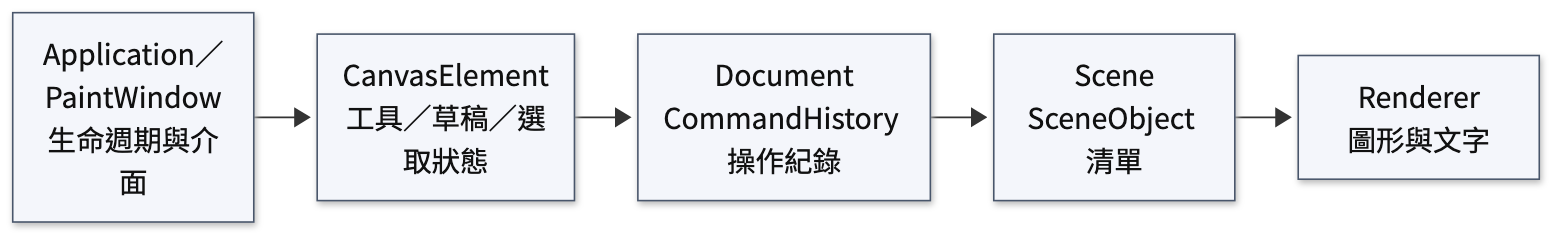
\includegraphics[width=.96\textwidth]{docs/figures/ch03_architecture.png}
    \caption{繪圖程式的整體架構}
    \label{fig:architecture}
\end{figure}

\subsection{Application 與 Window}

Application 統一管理 Paint Window、Dialog 與圖片輸出視窗。由於 FreeGLUT 只接受 C-style callback，程式以 GLUT window ID 找回對應的 C++ Window 實體，再把事件交給後續元件；Menu 也以相同方式將整數 ID 對應到實際動作。Callback routing、視窗生命週期與 Modal Dialog 的完整設計收錄於附錄~\ref{app:gui}。

\subsection{Document、Scene 與 Shape}

Document 記錄檔名、Canvas 尺寸、Scene 與 Command History，是繪圖內容修改的入口。Scene 依照繪製順序儲存 SceneObject，其中 ShapeObject 包含 Point、Line、Rectangle、Ellipse、Path 與 Polygon，TextObject 則記錄文字位置、UTF-8 字串與文字樣式。

這樣分層之後，Scene 不需要知道 UI，也不會直接呼叫 OpenGL。繪圖工具完成時只產生一個 SceneObject，再由 Document 建立 Command 修改 Scene。SelectTool 則只保留目前選取物件的暫時狀態；刪除時回傳 RemoveObjectAction，由 Canvas 交給 Document 建立 RemoveObjectCommand。拖曳中的 draft 與選取範圍都留在 tool overlay，所以這些暫時內容不會進入 Scene，也不會多產生一筆 Undo 紀錄。

\subsection{Event 與 Input}

Window 會把 GLUT callback 整理成帶有 keyboard 與 mouse state 的 Event，再依 hit test、mouse capture 與 parent chain 傳遞。工具因此能用一致的介面判斷拖曳與 Shift 等狀態；完整的 bubbling、focus、capture 與 shortcut 規則見附錄~\ref{app:gui}。

\subsection{Command History 與 Undo/Redo}
\label{sec:command-history}

加入、插入、移除物件與清空畫布都會建立可復原的 Command。每筆紀錄保存操作前後的 state ID，Undo／Redo 在兩個 stack 間移動同一筆 Command；新的操作則清空 redo stack。刪除物件時另記錄其原始索引，使 Undo 能恢復正確的前後層級。圖~\ref{fig:command-history} 整理了資料流。

\begin{figure}[tbp]
    \centering
    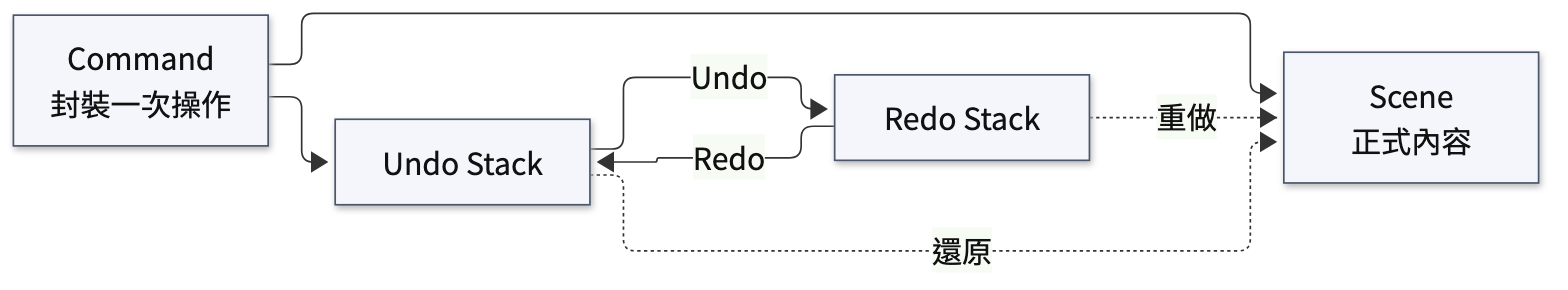
\includegraphics[width=.92\textwidth]{docs/figures/ch03_command-history.png}
    \caption{Command、復原與重做的資料流}
    \label{fig:command-history}
\end{figure}

\subsection{Rendering Pipeline}
\label{sec:rendering-pipeline}

Window 開始重繪時，Element tree 會按照各自的局部座標依序 render。輪到 Canvas 之後，CanvasRenderer 先畫 Grid，再按照 Scene 中的順序畫出物件，接著補上工具的 draft preview，最後在最上層畫選取範圍。SceneRenderer 會判斷物件是 Shape 還是 Text，再交給對應的 Renderer 呼叫 OpenGL。整條 Rendering Pipeline 如圖~\ref{fig:render-pipeline} 所示。

\begin{figure}[tbp]
    \centering
    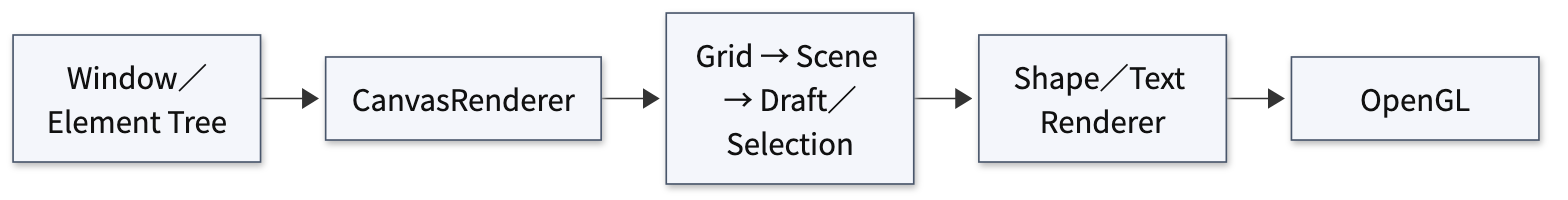
\includegraphics[width=.98\textwidth]{docs/figures/ch03_render-pipeline.png}
    \caption{目前的畫面渲染流程}
    \label{fig:render-pipeline}
\end{figure}
